\subsection{Product Perspective}
\subsubsection{Scenarios}
\begin{enumerate}
    \item \textbf{Educator Creates a Tournament} \newline Professor Emanuelle, a computer science educator giving an "Introduction to Programming" course in Politecnico di Milano, decides to improve her student's understanding of programming through coding exercises. She is already registered in CodeKataBattle as an educator, so she logs in to the platform with his credentials, which are her email and password. Then, she clicks the "Create Tournament" and a form screen is prompted. She fills out the form respectively: \newline
    - entering tournament title, "Winter Semester Coding Exercise 1", \newline
    - adding a description of the tournament, \newline
    - choosing a deadline for the subscription. After clicking the "Next" button\newline
    Professor Emanuelle is asked to select colleagues for permission to create battles in this tournament. She selects 2 of her colleagues because they all together give the same lecture. Finally, she clicks on the "Create" button, and the tournament is created. She is directed to the "My Tournaments" section after creation.
    \item \textbf{Student Registers for Tournament} \newline Emre is a Bachelor's student in Computer Science at Politecnico di Milano. At the start of the winter semester, he registered CodeKataBattle as a requirement of his "Introduction to Programming" course. In the middle of the semester, he gets an email notification about a tournament created by Professor Emanuelle on the platform. Then, He clicks the link in the email. Because he has already logged in to the platform with his email and password, he is redirected to the tournament's page, where he finds detailed information about Emanuelle's tournament. After reading the description, he thinks that this tournament will be very helpful for him to understand the topics covered in the lecture. So he clicks on the "Register" button to enroll tournament. Some registration details consisting of descriptions, educators, and tournament creator are shown on the screen. Also, he is informed that he will get email notifications for upcoming battles, battle rankings, and tournament rankings. Finally, Emre clicks on the "Accept and Register" button and registers the tournament.
    \item \textbf{Educator Sets Up a Battle} \newline A week ago Professor Mottola, was invited to a tournament created by his colleague in the CodeKataBattle platform. He accepted the invitation and learned about the tournament from its description. He also gives the "Introduction to Programming" course and wants to create a new exercise about the topic he showed in the last lecture, which is "Recursion". After the subscription deadline passed, he logs back into CKB, he selects the "Create Battle" option within the "Winter Semester Coding Exercise 1" tournament. He is presented with a detailed form where he inputs the battle's title, "Check if String is Palindrome" and provides a thorough description that includes the battle's focus on recursion, expected coding languages (Java and Python, both accepted), and software project including necessary scripts for build automation (Gradle for Java) and test cases. To encourage collaboration, he sets the minimum and maximum group size to three and five students, respectively. he then specifies the registration deadline, two weeks from the current date, and a final submission deadline, giving students a month to work on their solutions. Finally, he configures additional scoring parameters as \textbf{efficiency}, choosing from a list of aspects including reliability, maintainability, etc. Then he clicks on the "Create" button and he is redirected to battle main page illustrating information about the battle. After a couple of minutes, he got an email saying that an email about this battle was sent to all students in the tournament.\newline \newline
    \item \textbf{Student Joins for Battle} \newline Samet got a notification from the tournament he enrolled in saying that Professor Mottola has created a battle with the name "Check if String is Palindrome". He clicks on the link and reads the description carefully. He clicks on the "Register" button then a screen is shown asking Samet whether he wants to invite other students to form a team or not. Samet selects "Yes", then, he names her team 'Code Warriors' as a first step. Then he chooses students from a list of students registered for the tournament, considering minimum and maximum group size. Samet knows Emre, Jack, and Luca also registered for the tournament, so he sends them invitations. After clicking "Complete", he is redirected to the battle information page. On this page, there is a section showing group status, which is pending until all invitations are answered. After a while, Samet sees that Emre and Luca accepted but Jack rejected it. Because the minimum group size is fulfilled, Samet clicks on the "Finalize" button indicating the final decision. Thanks to the help of instructions during the process, Samet understands that if he wants to decline registration, he should have clicked on the "Decline" button. After every member accepts the invitation to finalize registration, the process ends and the status becomes "Registered". They are given a competitor id.
    \item \textbf{Students Sets Up Environment for CodeKataBattle} \newline With the 'Code Warriors' team formed and the registration deadline for the "Check if String is Palindrome" battle passed, the CKB platform takes its next automated step. It creates a unique GitHub repository for the battle, containing the provided code kata with its test cases and build scripts. The system then sends an email to Emre, Samet, and Luca with the repository link and instructions. The team members collaboratively decide to schedule a virtual meeting to set up their working environment. During the meeting, they fork the repository to their group account and set up GitHub Actions in order to make proper API calls with the competitor id they have. This setup is crucial for automating their workflow and ensuring that every code push not only updates their repository but also notifies the CKB platform. They test the setup by pushing a minor change, and upon seeing that the CKB platform acknowledges their commit, they know their system is correctly configured. This marks the start of their coding journey in the battle.
    \item \textbf{Students Solve Battle Challenge} \newline After forking the project and setting the environment, they started to think about the solution of the project. As they understand from the description they should return "True" or "False" regarding whether the given string is a palindrome. They implement the algorithm and commit/push the code to the repository. Each push prompts the platform to pull the latest code, run tests, and analyze the quality of their solutions using static analysis tools. After a while, they revisit the ranking on the battle's page to see their score for the last push. They see their scores in 3 different categories: \newline
    - functional aspects: 32/80 (4/10 test cases passed) \newline
    - timeliness: 5/5 \newline
    - quality level of the sources: 8/10 (Aspects: Efficiency) \newline
    In the rankings, they are informed via tooltips about the scaling of their scores and the calculation methods of them. So they decided to focus more on code and try to find why some test cases are not passed. The team keeps an eye on the CKB dashboard, which updates their battle score after each commit. They note improvements in their score as they refine their solutions, ensuring more test cases pass and optimizing their code for better quality. This iterative process of coding, committing, and refining continues, with the team members frequently discussing strategies and sharing insights to improve their solutions. After looking at some exercises related to recursions they finally found the wrong part in the algorithm they implemented. After changes they commit and push the code. They see in the rankings that they got 93 points from battle. This iterative process of coding, committing, and refining continues, with the team members frequently discussing strategies and sharing insights to improve their solutions. They think that this is the most efficient algorithm they can implement. So they decide not to do anything else until the battle deadline. \newline
    \item \textbf{Educator Evaluates Submission Manually} \newline
    After the submission deadline expires, there is a consolidation stage enabling educators to assign optional points for teams. Professor Mottola begins her manual evaluation of the submissions for the "Check if String is Palindrome" battle. He logs into CKB and accesses the educator's dashboard from the battle's page, where he can review each team's submission. On this page code of the submission and other materials from the repository are shown to the educator. He starts from the latest submission and gives extra points if he finds the solution by analyzing 'Code Warriors', impressed by their timely submission and high score, viewable in the rankings table. Professor Mottola examines their code, focusing on the efficiency of their solution, which got 8/10 from the analysis tool. Considering these factors, she awards them a high personal score. This score reflects her assessment of their problem-solving skills and coding proficiency, adding a crucial human element to the automated evaluation. 
    \item \textbf{Educators Analyse Tournament Leaderboard} \newline
    Professor Emanuelle created a tournament called "Winter Semester Coding Exercise 1" at the beginning of the semester. Some other colleagues of hers registered for the tournament as educators and created battles during the semester. During the semester, she has viewed the leaderboard and at the end of every week, she has exported the result. Eventually, at the end of the semester, Professor Emanuelle closes the tournament. She then goes to the leaderboard screen and starts to see the general success of her students by comparing leaderboard exports from the very first battle. In this way, she notices that the leaderboard becomes more competitive as we get closer to the end of the year. She interprets this situation as students improving their programming skills battle by battle. After analyzing the leaderboard she searched other ongoing tournaments of other professors from the university to see the success of their students in different tournaments created by teachers of different courses.
    
\end{enumerate}


\newpage
\subsubsection{Domain Class Diagram}
In the figure below, the Domain Class Diagram for the CodeKataBattle (CKB) platform is illustrated. This diagram is a crucial element in understanding the structure of the classes and relationships within the CKB system. It visually represents the key classes, their attributes, and the interactions among them in the context of the platform. This diagram is designed to provide a clear and concise overview of the domain model, offering insights into how the different components of the CKB platform interact to facilitate a competitive and educational coding environment. 

\begin{figure}[H]
    \centering
    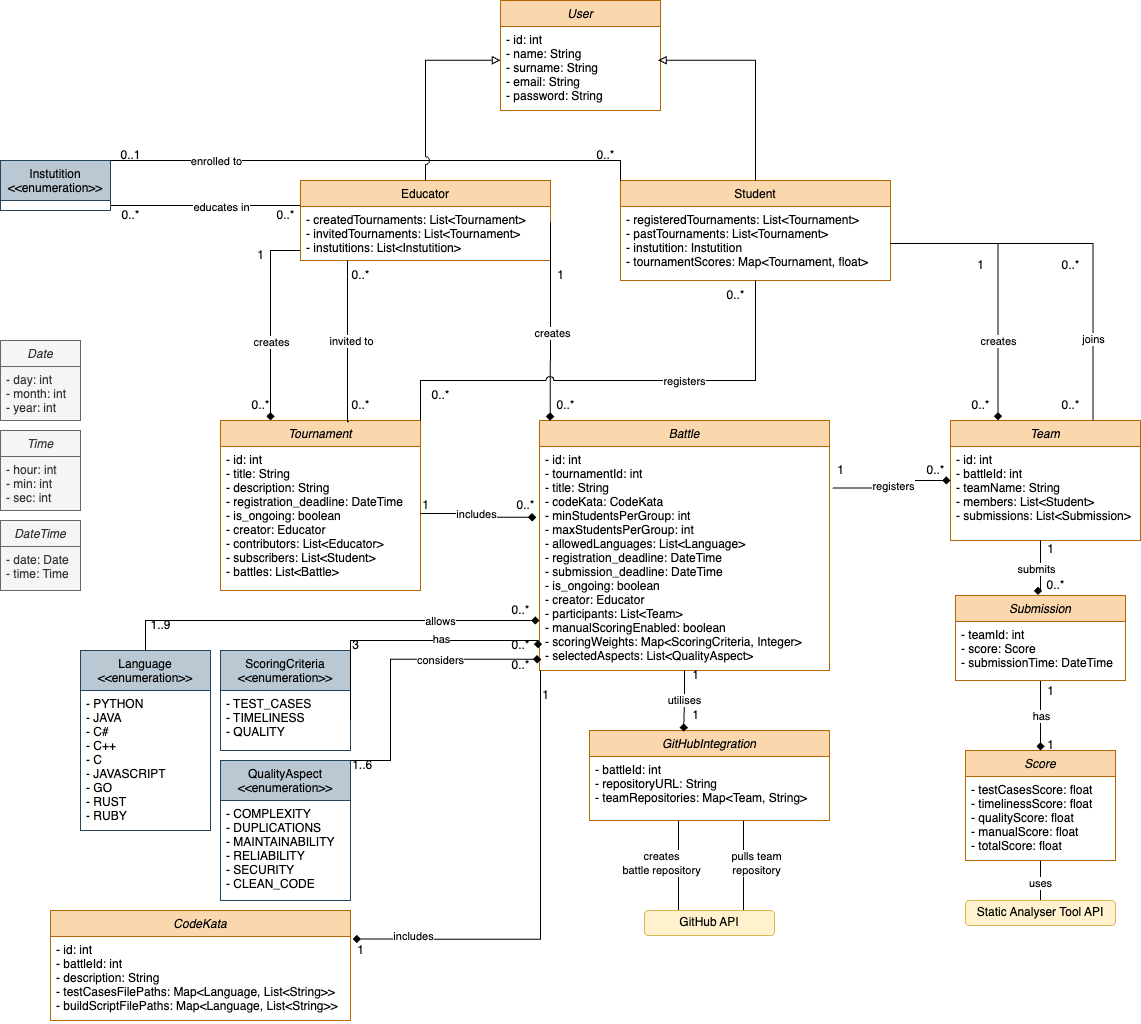
\includegraphics[width=\textwidth,height=\textheight,keepaspectratio]{Images/domainclassdiagramfinal.drawio.png}
    \caption{Domain Class Diagram}
    \label{fig:dcd}
\end{figure}


The descriptions below are the explanations of the important classes that take place in the diagram:
\begin{itemize}
    \item \textbf{User:} Serves as a base for different types of users. It encapsulates common attributes that are shared across students and educators. This class is essential for authentication.

    \item \textbf{Educator:} The objects of this class have the ability to create tournaments and battles. They can also be invited to a tournament by the creator of that tournament. 

    \item \textbf{Students:} The objects of this class have the ability to register for the tournaments, and they can create teams for battles or join teams that they are invited to.

    \item \textbf{Tournament:} Tournaments are a vital part of the project. They are created by educators and they include coding battles for teams of students to engage and solve.

    \item \textbf{Battle:} Battles are created by educators who take part in a tournament. During battle creation, educators set some of the fields of the battle object.

    \begin{itemize}
        \item \textbf{Scoring Criteria:} There exists 3 scoring criteria whose percentages are decided by the educator during battle creation.

        \item \textbf{Language:} There are 9 languages allowed in the system. The educator chooses the allowed languages during battle creation. At least one language must be chosen.

        \item \textbf{Quality Aspect:} There are 6 quality aspects that can be selected by the educator during battle creation time. At least one quality aspect must be chosen.

        \item \textbf{CodeKata:} It is the most important part of the battle. The test cases and the build scripts for each allowed language should be uploaded by the educator to the system. The paths to the files in the file system are stored in the fields.
    \end{itemize}

    \item \textbf{Team:} Teams are created by students, and the teams are able to register for the battles. They have a score for the battle.

    \item \textbf{GitHub Integration:} This class has one object for each battle and it stores the link to the GitHub repository for the battle after creating it by interacting with the GitHub API. It also stores the links to the repositories of the participating teams after they push their code and trigger a function that belongs to this class.

    \item \textbf{Submission}: Submissions are delivered by teams registered to battles. They have submission time and score of the submission.

    \item \textbf{Score:} The score of a team for each criterion is calculated for the battle. This class uses an external Static Analyser Tool to calculate the score of the quality aspect of the code. The timeliness and test case scores are handled internally.
\end{itemize}

\newpage
\subsubsection{Statecharts}
The state charts presented in this section elucidate the operation of the CodeKataBattle (CKB) project, illustrating the state transitions for a code kata battle and a tournament within the platform. Especially for tournaments, a state chart is very crucial to gain a better understanding of the tournament.\newline
\textbf{Tournament}

\begin{figure}[H]
    \centering
    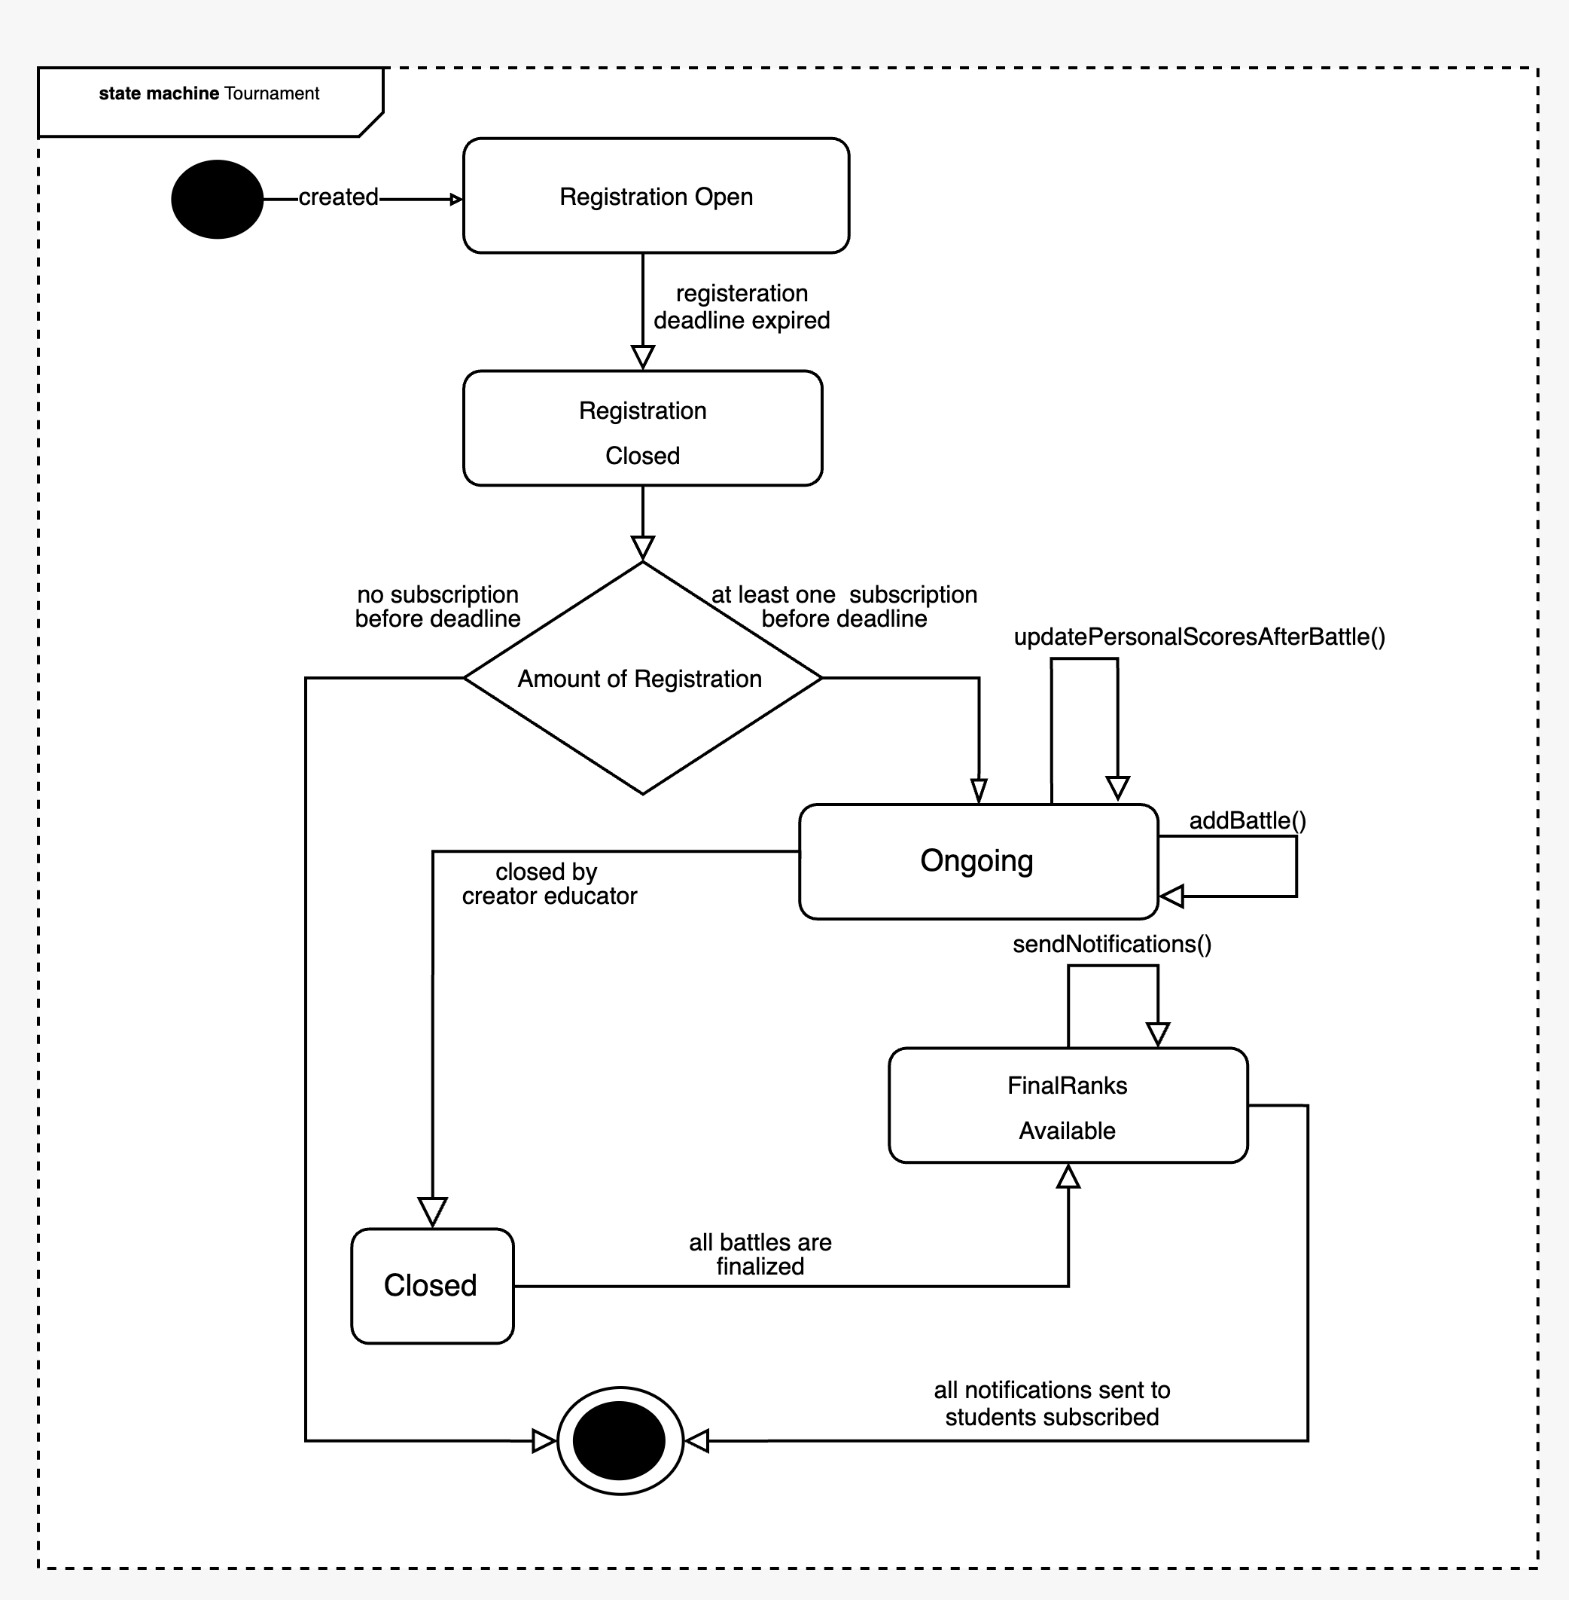
\includegraphics[scale=0.2]{Images/state_diagram/state_diagram_tournament.jpeg}
    \caption{$SC_{1}$ - Tournament}
    \label{fig:sc-t}
\end{figure}

Firstly, the tournament is in the very first state called "Registration Open", which indicates that Tournament is created and registration is open for students and invited educators. Until the registration deadline, they can register. When the deadline expires registration is closed, so the tournament goes into the "Registration Closed" state. In this state, the process controls the amount of registration for the tournament. If there is no registration it goes to "Final" state. Otherwise, the tournament starts with the "Ongoing" state. In this state, throughout the tournament, educators can create battles, and personal scores are updated after every battle. If the creator educator closes the tournament, it goes to the "Closed" state. However, there can be some battles in the consolidation stages and it is mandatory to finalize them to calculate final ranks. After every battle is finalized, the tournament transitions to the "FinalRankAvailable" state in which notifications about final rankings are sent to the students. After finishing this notification process tournament reaches the "Final" state. There won't be any rank changes or notifications hereafter. \newpage
\textbf{Battle}\newline

\begin{figure}[H]
    \centering
    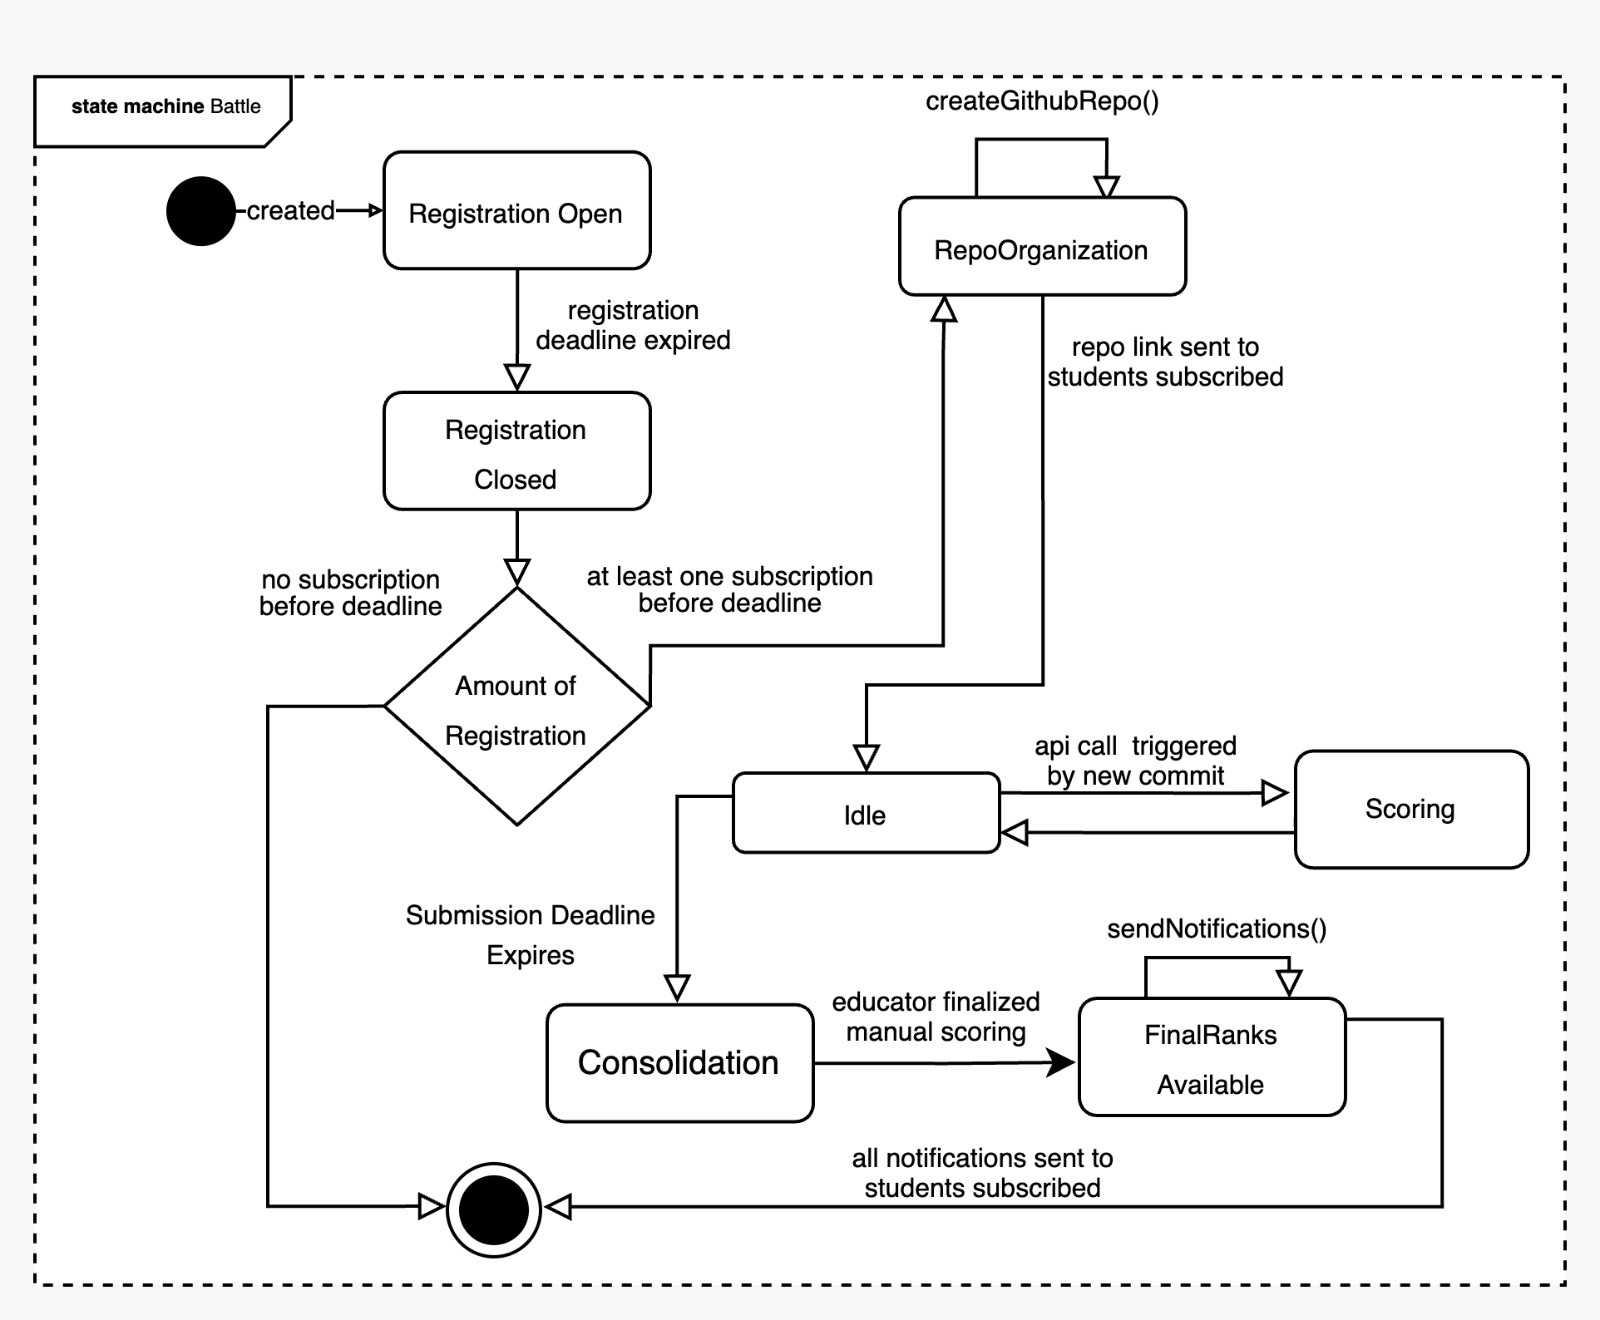
\includegraphics[scale=0.2]{Images/state_diagram/state_diagram_battle.jpeg}
    \caption{$SC_{2}$ - Battle}
    \label{fig:sc-b}
\end{figure}

Firstly tournament is created with the "Registration Open" state. In this state, students can register to battle with teams or individually. When the deadline expires, Battle goes into the "Registration Closed" state. At this time, it is calculated that if there is any registration for battle. If no, it goes to the "Final" state with no registration and any other action. If there are registrations, it goes to a new state called as RepoOrganization in which GitHub repository for the battle is created with proper instructions. Sending the link and instructions triggers the process to go into the "Idle" state. This means that Battle has started and waits for API calls from forked repositories, triggered by a new commit. An API call from repositories of competitor leads to scoring phase. Until the submission deadline, battle switches between Scoring and Idle states.Eventually, it returns to the "Idle" state. Until the submission deadline, students' commit can change their scores. When the deadline expires, Battle goes into the "Consolidation Stage" state in which educators can change rankings via manual scorings. When they are finalized, Battle is closed, indicating as state "FinalRanksAvailable". Immediately, the notification sending process starts. After all notifications are sent, Battle goes into the Final state.
\newpage
\textbf{Submission}\newline

\begin{figure}[H]
    \centering
    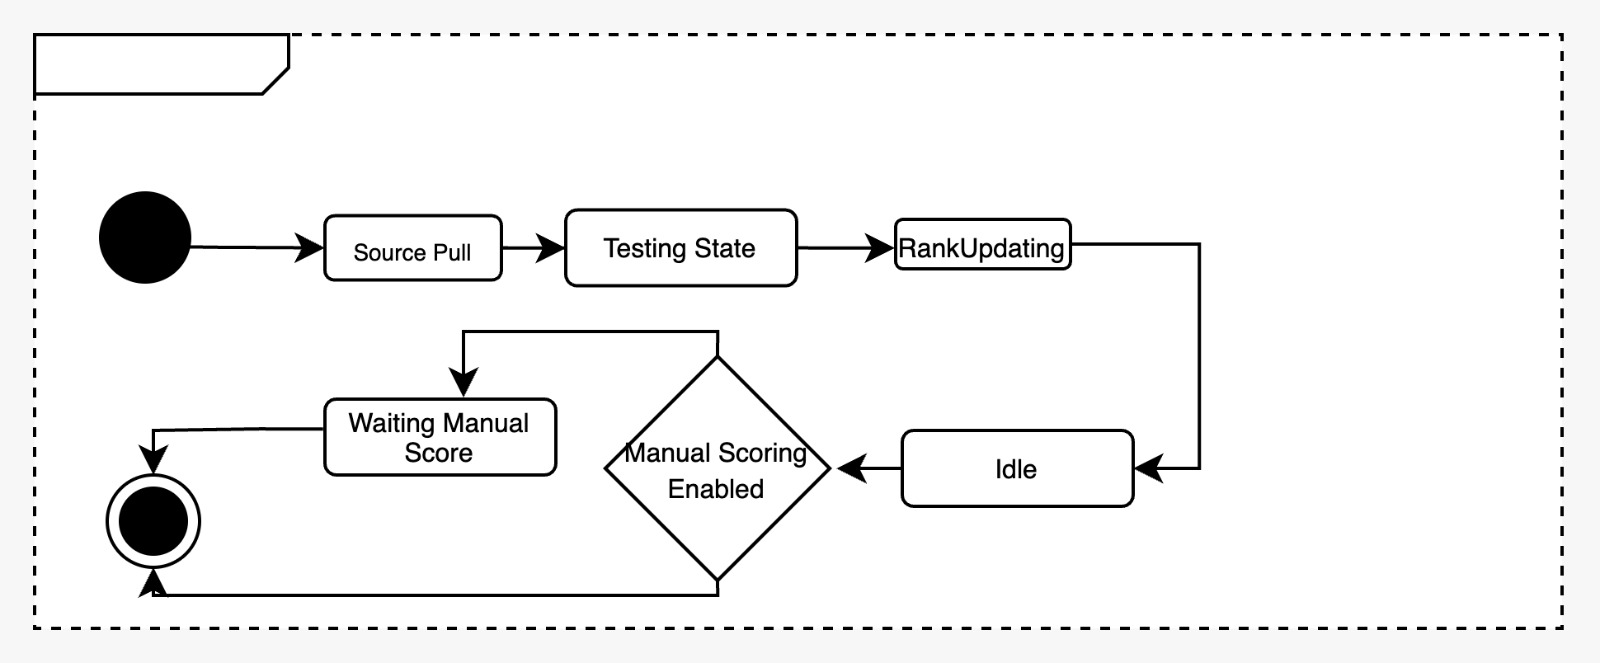
\includegraphics[scale=0.2]{Images/state_diagram/state_diagram_submission.jpeg}
    \caption{$SC_{3}$ - Submission}
    \label{fig:sc-s}
\end{figure}


Firstly, Submission goes into source pulling and initialization phases. After Testing and Rank Updating, which are sequential phases, submission become idle until the submission deadline. In there, either it goes into consolidation stage for manual scoring or immediately finalized. rankings are updated.
\newpage

\subsubsection{Activity Diagrams}
\textbf{Register Battle}
\begin{figure}[H]
    \centering
    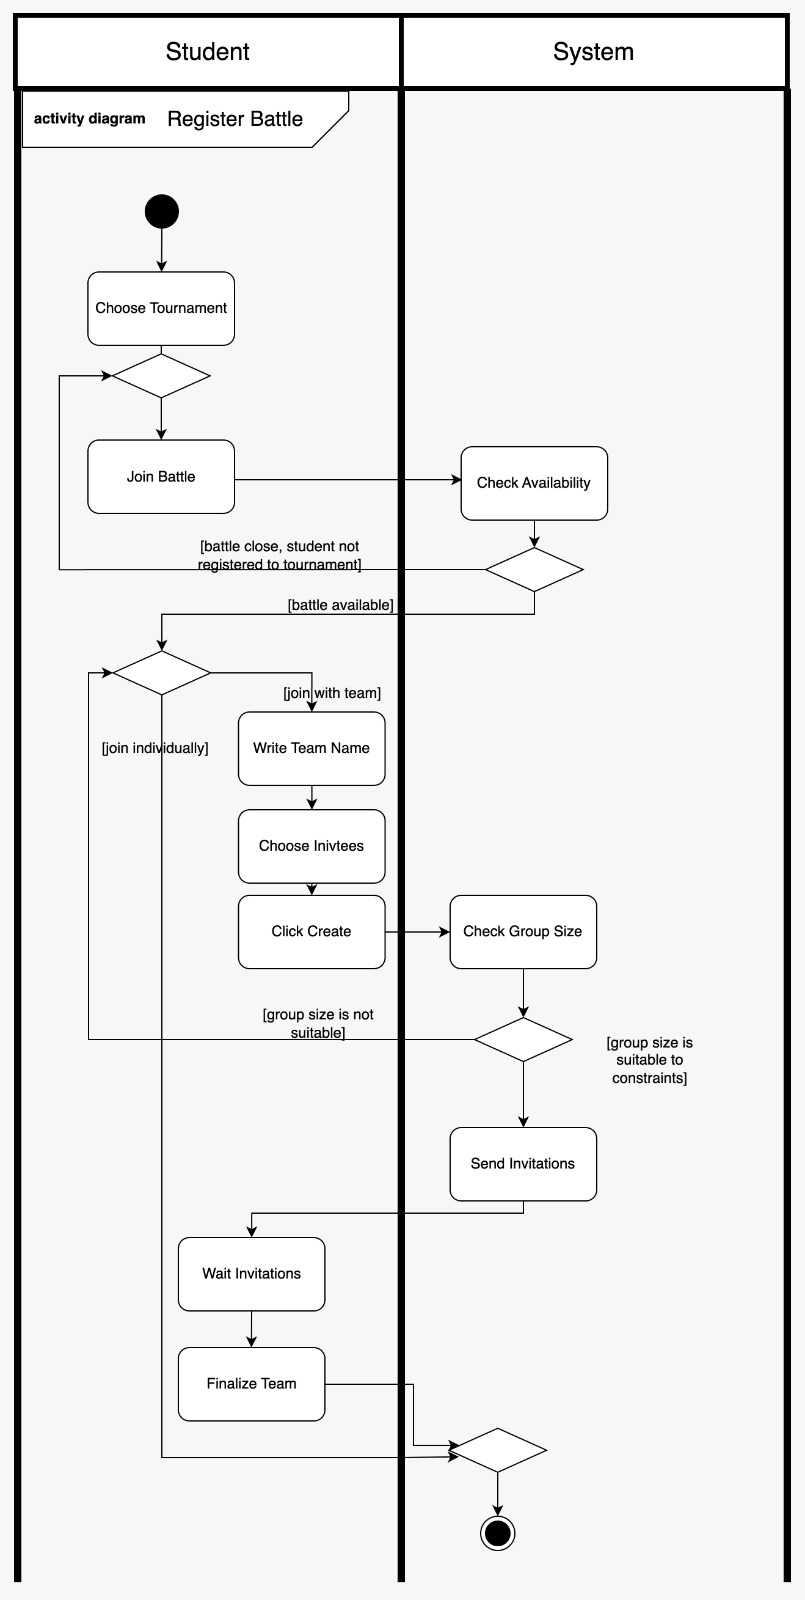
\includegraphics[scale=0.27]{Images/activity_diagram/activity_diagram_register_battle.jpeg}
    \caption{$AC_{1}$ - Register Battle}
\end{figure}


\newpage
\textbf{Create Battle}
\begin{figure}[H]
    \centering
    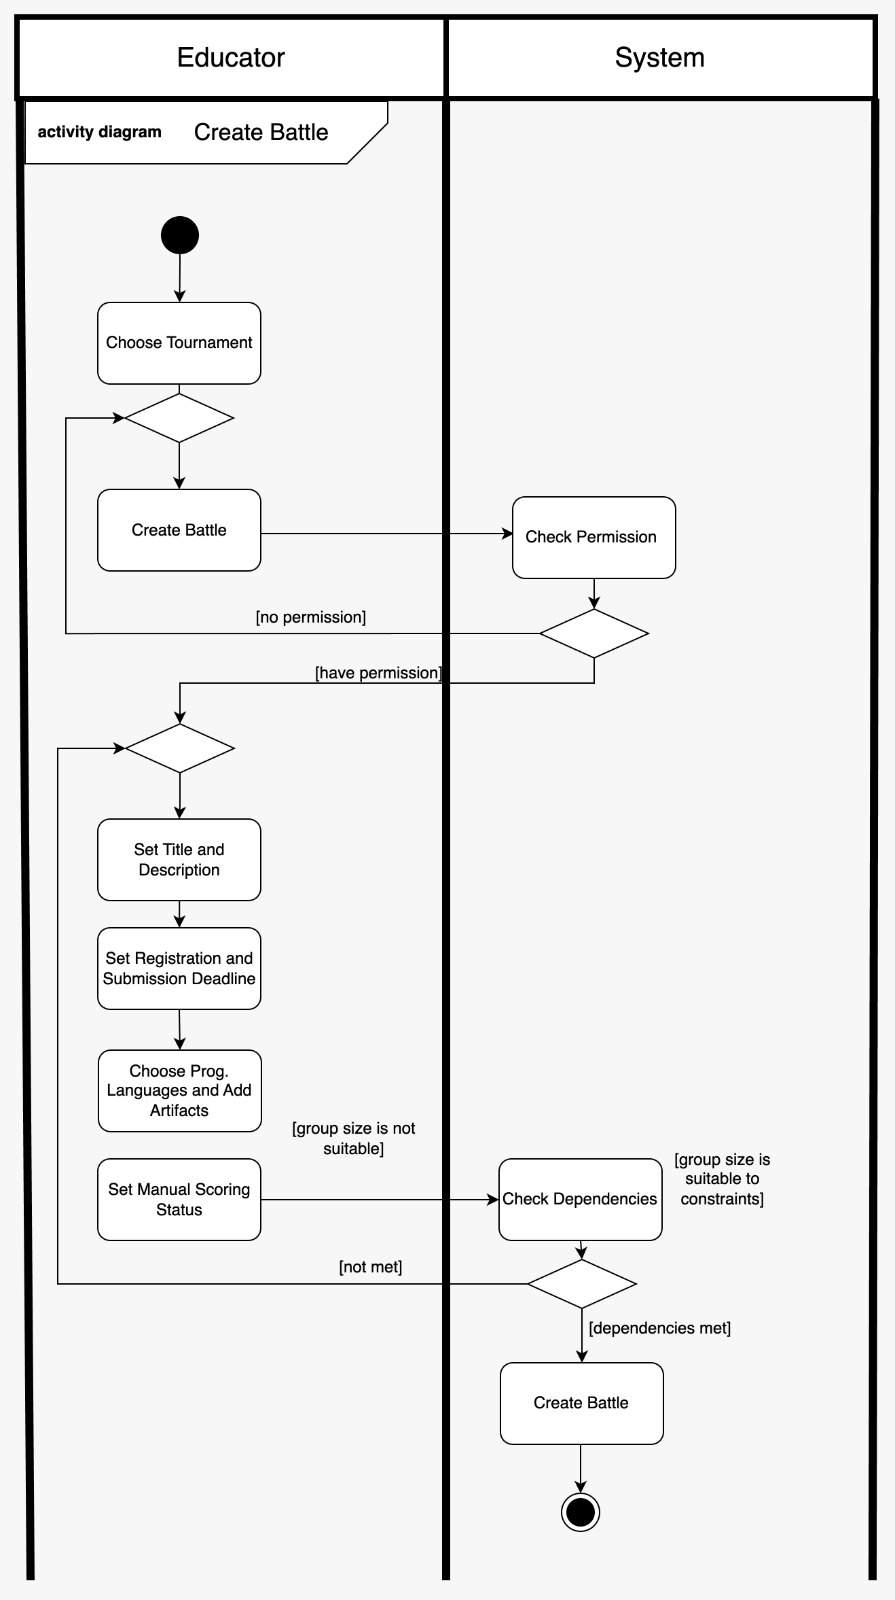
\includegraphics[scale=0.327]{Images/activity_diagram/activity_diagram_create_battle.jpeg}
    \caption{$AC_{2}$ - Create Battle}
\end{figure}

\newpage
\textbf{Submission}
\begin{figure}[H]
    \centering
    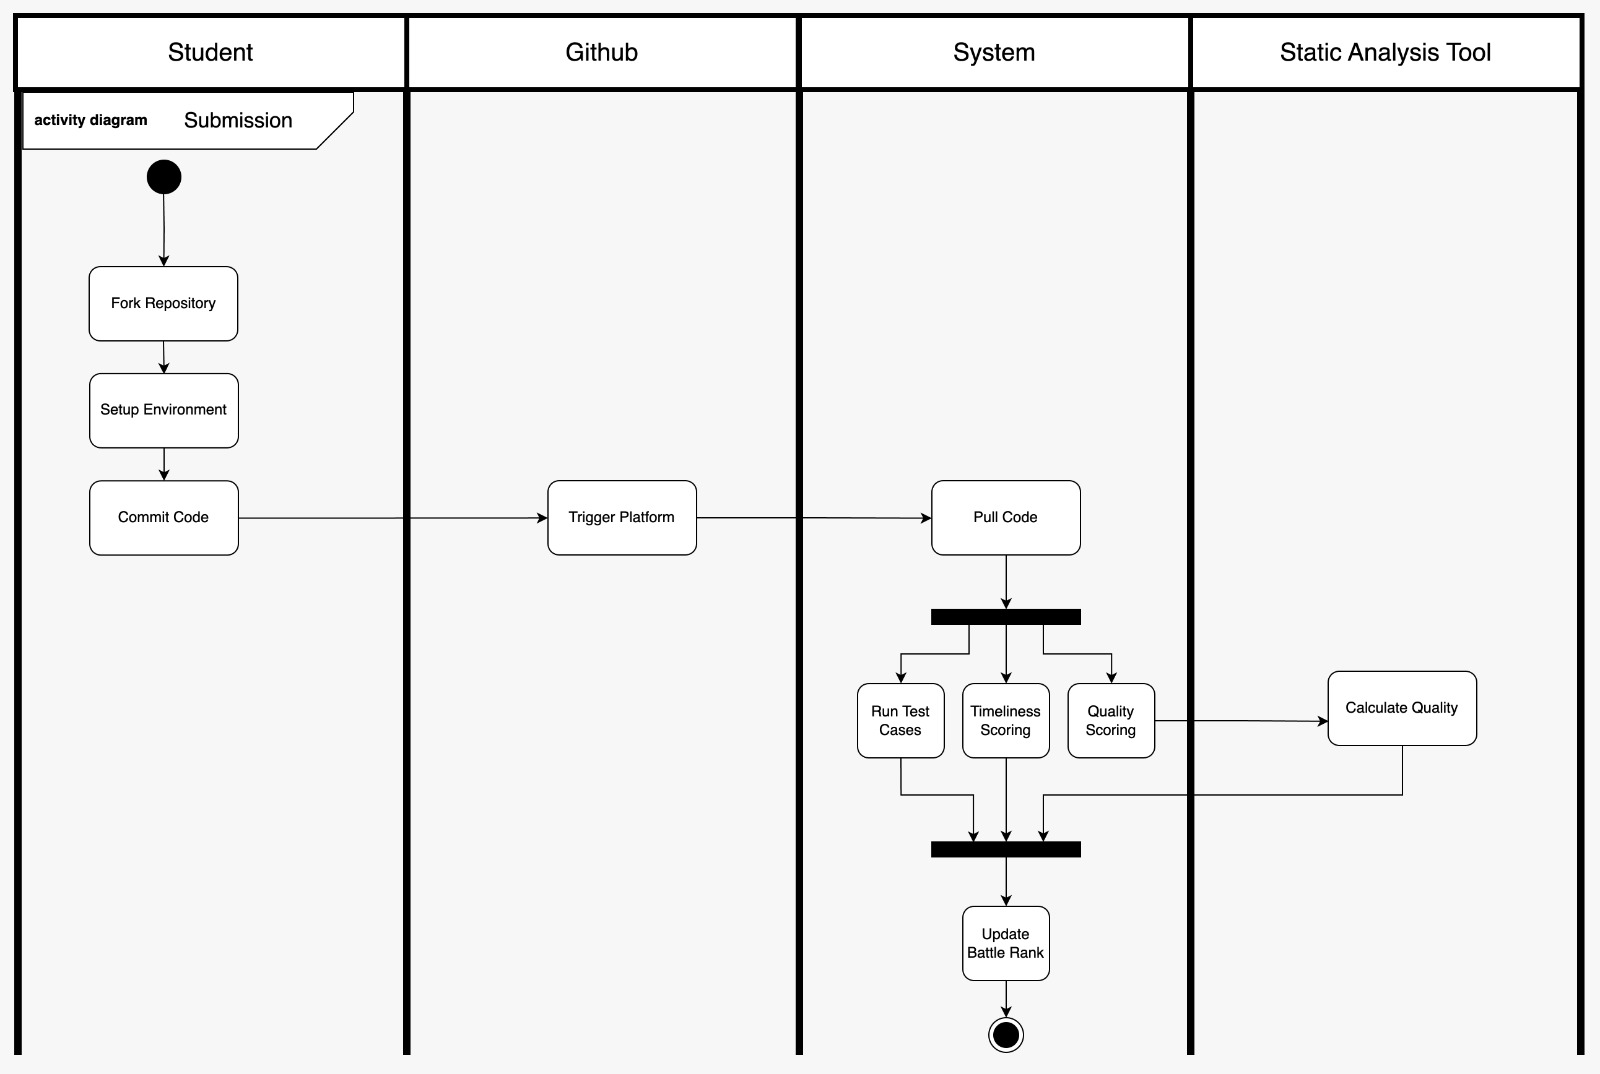
\includegraphics[scale=0.27]{Images/activity_diagram/activity_diagram_submission.jpeg}
    \caption{$AC_{3}$ - Submission}
\end{figure}

\newpage
\subsection{Product Functions}

The major functions of the project will be organised according to the user types. We will have three sections, first for the common function both regarding the educators and the students. The second and the third will be specific to each user type respectively.

\subsubsection{Common Functions}

\begin{itemize}
    \item \textbf{Account Registration:} Both students and educators can be registered to the platform. During registration, the user indicated which type of user they are along with their credentials.

    \item \textbf{Viewing Leaderboards and Rankings:} Both user types can view leaderboards that display rankings of participants based on performance in battles and overall tournament standings.
\end{itemize}

\subsubsection{Educator Functions}
\begin{itemize}
    \item \textbf{Creating a Tournament:} Educators can create and configure tournaments, setting specific parameters such as time constraints. In these tournaments, multiple battles can take place.

    \item \textbf{Creating a Battle:} Educators can create and configure coding battles in the tournament that they have created or they have been permitted by their fellow educators. During battle creation, specific parameters such as coding languages, and team sizes are set by the educator. On top of that, the description of the battle and the test file including test cases, automated build scripts or manual evaluation choice should be provided.

    \item \textbf{Giving Permission to Other Educators:} This function can be utilised both in the creation of a tournament and during the management of a tournament. Educators are able to permit fellow educators to create battles in the tournaments that they have created.

    \item \textbf{Scoring:} This function is vital since it is used to compute the points of the students' submissions in the battles. The output of this method determines the ranking of the students. Both automated and manual scoring reply to this function call.
    
\end{itemize}

\subsubsection{Student Functions}
\begin{itemize}
    \item \textbf{Join a Tournament:} Students can join tournaments that the educators are created. When they join a tournament, they will be able to take part battles in it.

    \item \textbf{Join a Battle:} Students can join battles which is a part of the tournament they already joined. When joining the battle, students can send requests to other students to form a team if they want or need to.

    \item \textbf{Send Request for Teaming:} This function can be called during students join the battle. Students send requests to other students using their usernames, and if they accept the invitation, they are now a part of the team for the battle they are joining.

    \item \textbf{Submit Solution:} Students submit their solutions for each code battle. After submission successfully completed, the scoring function is called.
\end{itemize}





\newpage
\subsection{User Characteristics}

\subsubsection{Educators}

\begin{enumerate}[A.]
    \item \textbf{Profile}

        \begin{itemize}
            \item Typically instructors, professors, or teachers in computer science or related fields, with varying levels of experience in coding and software development education.
        \end{itemize}

    \item \textbf{Needs}

        \begin{itemize}
            \item Tools for creating, managing, and monitoring coding challenges and tournaments.
            \item Flexibility in setting parameters for battles, including team sizes, deadlines, and testing criteria.
            \item Ability to assess student work both automatically or manually.
            \item Resources to track student progress and engagement in coding exercises.
        \end{itemize}

    \item \textbf{Interactions}

        \begin{itemize}
            \item Making students engage with battles for educational purposes.
            \item Collaboration with other educators within or across institutions.
        \end{itemize}
    
\end{enumerate}

\subsubsection{Students}

\begin{enumerate}[A.]
    \item \textbf{Profile}

        \begin{itemize}
            \item Individuals enrolled in computer science and similar courses or those seeking to enhance their coding skills, ranging from beginners to advanced levels.
        \end{itemize}

    \item \textbf{Needs}

        \begin{itemize}
            \item Access to a variety of coding challenges that help to improve the student's skills.
            \item Tools for collaborative coding and team formation.
            \item Real-time feedback on code submissions for iterative learning.
            \item Opportunities to apply theoretical knowledge in practical scenarios.
        \end{itemize}

    \item \textbf{Interactions}

        \begin{itemize}
            \item Active participation in coding battles and tournaments.
            \item Collaboration with peers for team-based challenges.
            \item Utilisation of platform resources for self-directed learning and improvement.
        \end{itemize}
    
\end{enumerate}


\newpage
\subsection{Assumptions, Dependencies, and Constraints}

\subsubsection{Domain Assumptions}

\begin{enumerate}
    \item Educators and students have basic proficiency in using web-based platforms and are familiar with basic operations such as account creation, logging in, and navigating through a digital interface.

    \item Educators have the necessary skills to create and manage coding challenges, including the ability to correctly write problem descriptions, test cases, and understand code quality metrics.

    \item The coding problems and challenges provided by educators are free from errors and ambiguities.

    \item Students have at least foundational knowledge in programming and can understand and respond to coding challenges.

    \item Students' submissions to the platform are their original work.

    \item The users have access to reliable internet connectivity and devices capable of supporting the web-based CKB platform.

    \item Students have familiarity with GitHub operations such as forking a repository, setting up GitHub Actions, and committing and pushing their codes.

    \item The automated testing and scoring systems within the CKB platform are trusted by users to fairly and accurately assess coding submissions. Similarly, educators are trusted in the case of manual evaluation of submissions.

\end{enumerate}

\subsubsection{Dependencies}

\begin{itemize}
    \item \textbf{GitHub Services:} The system's functionality for code submission and automated workflow relies on the availability and reliability of GitHub services.

    \item \textbf{Static Analyser Tool:} The system's functionality for code evaluation on quality aspects relies on the availability of an external API that provides Static Analysis.

    \item \textbf{Internet Connectivity:} Access to the internet is essential for both users.

    \item \textbf{Web Browser Compatibility:} The platform's user interface and features depend on their compatibility with various web browsers, ensuring all users can access and use the platform effectively.

    \item \textbf{Hosting Services:} Dependence on reliable hosting services (like cloud-based servers) for hosting the web application, database, and related services.

    \item \textbf{Notification Service:} The platform depends on an external notification service to send timely alerts and updates to students and educators.

    \item \textbf{Email Verification Service:} The platform relies on an external email service provider to send verification codes to users during the account registration process.

    
\end{itemize}


\subsubsection{Constraints}

\begin{itemize}
    \item \textbf{Technological Constraints:} Compatibility requirements with various web browsers and devices may limit certain design or feature implementations.

    \item \textbf{Resource Constraints:} Hosting and operational costs may limit the extent of scalability and redundancy features of the platform.

    \item \textbf{Security and Privacy Constraints:} The system must adhere to strict data protection and privacy regulations, such as GDPR, which may limit certain data collection and processing activities.

    \item \textbf{Legal and Compliance Constraints:} Compliance with intellectual property laws, particularly in the use and distribution of coding challenges and educational content, i.e. the rights of the contents are reserved.
\end{itemize}